\label{referencial}
\section{Metodologias Ágeis}

% -- O mundo hoje em dia está muito rápido, e as mudanças ocorrem de maneira muito rápida


% -- Explicação do modelo anterior, e suas desvantagens
Desde o surgimento da disciplina de Engenharia de Software em 1968, o desenvolvimento de software seguiu os processos enunciados em modelos não iterativos, ou seja, planejados. Um deles é o modelo em cascata, em que a saída de cada fase do processo de desenvolvimento é a entrada para a outra fase, de uma maneira linear. Várias desvantagens foram vistas como por exemplo planejar todo o processo de desenvolvimento, com requisitos que se mantêm estáveis do começo ao fim do desenvolvimento. Além disso, em um projeto complexo, requisitos definidos em sua fase inicial, poderia levar a um produto não mais necessário, depois de anos de desenvolvimento, em que os requisitos atuais já são bem distintos dos iniciais \cite{sommerville2015software}. Também é considerado uma desvantagem o overhead em planejar, projetar e documentar o sistema no modelo tradicional, fazendo com que o software seja desenvolvido e entregue apenas após as fases anteriores sejam cumpridas \cite{sommerville2015software}.

% -- Necessidade do modelo ágil, e suas vantagens
Os métodos ágeis são métodos de desenvolvimentos incrementais, com entregas pequenas, em curtos períodos de tempo como semanas. A ideia é a entrega de software útil rapidamente, envolvendo os clientes no desenvolvimento para acelerar o feedback, verificando se aquilo que está sendo entregue é aquilo que estava sendo esperado pelo cliente, minimizando documentação \cite{sommerville2015software}.
O desenvolvimento ágil é vantajoso em ocasiões em que a equipe é de pequena a médio porte, e o software a ser desenvolvido é personalizado. Por exemplo em uma companhia pequena a médio porte, em que se está produzindo um software sob medida para um cliente, seria interessante mostrar entregas incrementais, além do que cliente poder verificar junto com a equipe de desenvolvimento o que se está sendo produzido, este poderia mudar os requisitos de acordo com suas necessidades, que se alteram durante o tempo \cite{sommerville2015software}.


% -- O Manifesto ágil e o que todas compartilham em comum
Apesar dos diferentes métodos ágeis se basearem em diferentes processos ágeis, um conjunto de princípios é compartilhado entre eles, com base no Manifesto Ágil. O desenvolvimento e as entregas de software devem serem feitas incrementalmente. A Tabela X mostra os princípios compartilhados em comum entre as diferentes metodologias.

Inserir Tabela
Princípio - Descrição
Envolvimento do cliente
Os clientes devem estar presentes durante todo o processo de desenvolvimento, provendo e priorizando novos requisitos de sistema e avaliando as iterações do sistema.

Incorporação de mudanças
Projetar o sistema para acomodar mudanças, pois é esperado que os requisitos mudem.

Entrega incremental
Os clientes especificam os requisitos a serem incluídos em cada incremento, assim o software é desenvolvido de maneira incremental.

Manter simplicidade
O processo de desenvolvimento e o software devem caminhar com foco em simplicidade, sendo sempre que possível feita a eliminação de complexidade do sistema.

Pessoas, não processos
Os times devem desenvolver suas próprias maneiras de trabalhar, assim reconhecendo e explorando as habilidades do time de desenvolvimento.

Caption: Princípios das metodologias ágeis \cite{sommerville2015software}.


% -- Quais são as técnicas mais usadas

% -- Pq usar o Scrum em vez das outras Gerenciamento de Projeto Ágil
% Devo colocar as terminologias do Scrum?

Scrum é uma metodologia ágil que provê um framework para organizar projetos ágeis \cite{sommerville2015software}. O ponto central do Scrum está nas Sprints, que são entregas incrementais do sistema a ser desenvolvido em um período de tempo pré fixado. A atividade de planejamento no Scrum é fundamentada em priorização do backlog -- que é um conjunto de User Stories, atividades a serem desenvolvidas pelo time de desenvolvimento -- e a seleção de uma tarefa com prioridade alta para uma Sprint \cite{sommerville2015software}.


% -- Dificuldade de Metodologias Ágeis em relação a REQUISITOS
Apesar de suas vantagens, ao tratar requisitos os métodos ágeis não criam documentos de requisitos coerentes, pois coletam requisitos informalmente e de maneira incremental \cite{sommerville2015software}, podendo dificultar a manutenção do sistema.

% -- Exemplo de User Stories / com privacidade incluída, né
TO-DO

\section{Elicitação de Requisitos}
%cabe subseções : Fontes de Requisitos , Técnicas de Elicitação de Requisitos

% -- Definição Requisitos e Engenharia de Requisitos
Os requisitos são o reflexo das necessidades dos clientes para um sistema, que devem servir para um propósito (e.g., traçar a rota mais rápida no mapa, não divulgar os dados dos usuários a terceiros). Os requisitos para um sistema são definidos como a descrição dos serviços que um sistema deve fornecer, além das restrições ao seu funcionamento \cite{sommerville2015software}. 
% -- Classificações de Requisitos (Funcionais e não funcionais)
Requisitos são definidos por clientes, que muitas vezes não possuem conhecimento técnico necessário para alcançar um alto nível de detalhamento do requisito a ser levantado. Por tanto, existem diferentes níveis de descrição de requisitos. Sommerville \cite{sommerville2015software} distingue entre requisitos do usuário e requisitos do sistema, afim de evidenciar esse fato. 

Requisitos do usuário são descrições em linguagem natural, de alto nível e abstratas, do que o usuário espera que os serviços do sistema possam fornecer, além de restrições em que ele deve operar \cite{sommerville2015software}. Requisitos do sistema são descrições mais detalhadas, devendo definir exatamente o que é a ser implementado, como funções, serviços e restrições operacionais \cite{sommerville2015software}. Essa necessidade de níveis diferentes de detalhamento ao descrever requisitos acontece porque diferentes tipos de leitores utilizam eles de várias maneiras.

Além da distinção entre os níveis de detalhamento dos requisitos apresentada, estes são classificados em dois grupos: requisitos funcionais e requisitos não funcionais.
Os requisitos funcionais são declarações do que o sistema deve prover, e como deve reagir e se comportar a situações particulares, além do que não deve fazer \cite{sommerville2015software}.

Os requisitos não funcionais geralmente descrevem restrições nas funcionalidades ou serviços de um sistema (e.g., o tempo máximo de consulta não deve exceder 5 segundos, o sistema não pode ficar mais que 5 minutos fora do ar em um dia).  

Sem embargo, não há uma separação precisa entre os tipos de requisitos, revelando que os requisitos não são independentes um dos outros, e que um pode gerar ou limitar outros requisitos. No caso de um requisito de usuário relacionado com segurança, como limitar o acesso somente à usuários autorizados, que podem aparecer como um requisito não funcional, ao ser desenvolvido com um grau maior de detalhamento pode gerar requisitos que são funcionais, como a necessidade da inclusão do serviço de autenticação do usuário no sistema \cite{sommerville2015software}.

Referir-se aos processos de identificar, analisar, documentar e verificar esses serviços e restrições, é definir a Engenharia de Requisitos (ER) \cite{sommerville2015software}. 

% -- Processos da Engenharia de Requisitos
A Engenharia de Requisitos geralmente é visto como o primeiro estágio do processo de engenharia de software \cite{sommerville2015software}. 

São três as principais atividades envolvidas na ER: elicitação e análise -- descoberta de requisitos ao se interagir com os clientes; especificação -- conversão dos requisitos em uma forma padrão; validação -- checagem que os requisitos realmente definem o sistema que o cliente quer. Estes processos são iterativos e intercalados, produzindo ao final o documento de requisitos do sistema \cite{sommerville2015software}. Nesta dissertação, focamos na atividade de elicitação de requisitos em times ágeis.

% -- Elicitação de Requisitos ( SOMMERVILLE só trata no tradicional, mas ele tem umas paginas la no de agil)

Os objetivos da elicitação de requisitos são entender a) o trabalho que os clientes realizam, e b) como um novo sistema pode auxiliar este trabalho \cite{sommerville2015software}. 

A elicitação de requisitos compreende o conjunto de atividades que permitem a descoberta, compreensão e documentação dos objetivos, além dos motivos para o desenvolvimento de um sistema de software \cite{franco2016}. É durante esta fase -- de elicitação de requisitos -- que os engenheiros de software trabalham juntamente com os clientes, a fim de compreender questões relacionadas ao domínio de aplicação, atividades de trabalho, os serviços e características do sistema que são desejadas pelas partes interessadas, além de aspectos necessários como desempenho, privacidade, entre outros \cite{sommerville2015software}.

% -- Dificuldades enfrentadas durante o processo de Elicitação de Requisitos

As partes interessadas geralmente não sabem o que desejam de um sistema de computador, por serem na maior parte das vezes leigos, descrevendo em termos gerais e com dificuldade de expressar o que esperam. Dificuldade do engenheiro de software de compreender o domínio do usuário, devido a expressão das partes interessadas nos seus próprios termos, em que não se há (tampouco se espera) uma expertise prévia (e.g., um jurista descrevendo um sistema judicial). Como há diferentes partes interessadas e diferentes requisitos, o engenheiro de software deve saber descobrir as distintas fontes de requisitos, além de suas similaridades e diferenças. Pela natureza dinâmica, os fatores políticos e econômicos influenciam nos requisitos, às vezes por exigências específicas de gerentes ou por mudanças inevitáveis de requisitos que podem ocorrer durante esta fase. Assim, são várias as dificuldades percebidas e enfrentadas durante este processo \cite{sommerville2015software}.

Algumas técnicas de elicitação de requisitos são a) Entrevistas, b) Observações, c) Histórias e Cenários. Essas técnicas podem ser aplicadas em conjunto \cite{sommerville2015software}.

\subsection{Elicitação de Requisitos nas Metodologias Ágeis}

% -- Elicitação de Requisitos nas metodologias ágeis - Preâmbulo
No âmbito das metodologias ágeis, a Engenharia de Requisito é feita iterativamente e ao longo de todo o processo de desenvolvimento, se distinguindo da ER nos modelos tradicionais, que a possuem apenas como uma única fase no início de projeto \cite{FerreiraMartins2019}.

% -- User Stories (ou como se faz a atividade de Engenharia de Requisitos na metodologia ágil)

Para lidar com as mudanças -- visto que os requisitos de software estão em constante mudança --, os métodos ágeis não possuem uma atividade separada de Engenharia de Requisitos. A elicitação de requisitos é integrada ao desenvolvimento \cite{sommerville2015software}. A fim de facilitar esta atividade, foi desenvolvida a ideia de User Stories. A história de usuário é um cenário de uso que pode ser experienciado por um usuário do sistema \cite{sommerville2015software}.
Visto que desde o princípio o cliente está participando de perto do processo de desenvolvimento, este em conjunto com o time de desenvolvimento elaboram um story card, que descreve brevemente as necessidades do usuário. As histórias de usuário podem ser usadas nas iterações de planejamento do sistema, e, uma vez desenvolvida, é quebrada em tarefas pela equipe de desenvolvimento que então estima o esforço e recursos necessários para a implementação de cada tarefa \cite{sommerville2015software}. O refinamento dos requisitos é feito com os clientes e o time de desenvolvimento, o primeiro prioriza as Stories para implementação. Com o usuário participando e priorizando os user stories a serem implementados, as funcionalidades que são mais úteis e que agregam mais valor de negócio são identificadas e desenvolvidas primeiro, nas primeiras versões do sistema, ou seja, nas primeiras sprint cycles

% -- Dificuldades com User Stories
A principal desvantagem de se utilizar User Stories para se realizar a atividade de Engenharia de Requisitos nas metodologias ágeis é a dificuldade em se perceber se uma User Story está completa e identifica todos os requisitos essenciais de um sistema \cite{sommerville2015software}.


\section{Requisitos de Privacidade}

% -- Aquele artigo que faz uma especificação de requisitos de privacidade como Funcionais

\section{Privacidade By Design}


\section{LGPD versus GDPR}



\section{Design Thinking}



\section{Trabalhos Relacionados}


%Inicio do Cap 2 do Frederico
% De acordo com Wang et al. \cite{wang2016practical}, uma forma de selecionar e priorizar algoritmos de pesquisa baseados em Pareto seria por meio da priorização de indicadores de qualidade. Nesse sentido, o objeto de estudo dos autores apresenta um guia prático para selecionar indicadores de qualidade com o intuito de avaliar algoritmos de pesquisa baseados em Pareto em diferentes contextos da engenharia de software. O guia prático deriva dos seguintes itens complementares: 

% \begin{itemize}
%     \item Métodos teóricos e empíricos;
%     \item Fundamentos teóricos sobre os indicadores de qualidade;
%     \item Evidências da revisão de literatura;
%     \item Evidências coletadas de um experimento realizado para avaliar oito indicadores de qualidade de quatro categorias diferentes, com seis algoritmos de busca baseados em Pareto, utilizando três problemas reais de dois domínios diversos.
% \end{itemize}

% Marforio et al. \cite{marforio2016evaluation} propõem a definição de indicadores de segurança personalizados para mensurar determinados ataques maliciosos. Segundo os autores, indicadores de segurança personalizados podem ajudar os usuários a detectar ataques de \textit{phishing}, mas dependem da atenção do usuário.

% Com relação aos problemas relacionados ao escopo do projeto, as técnicas de priorização de indicadores precisam ser amplas o suficiente para estabelecer condições de definir uma lista de indicadores prioritários sob o ponto de vista do cliente, mas ainda deve se concentrar na definição de indicadores, caso o indicador a ser priorizado ainda não exista. Não entender problemas contextuais pode levar a indicadores incompletos, não priorizáveis, desnecessários e inutilizáveis. Concentrar-se em atividades de design mais amplas enfatiza os problemas dos desenvolvedores em relação às necessidades dos usuários e pode resultar em indicadores que expressam as reais necessidades dos clientes e usuários \cite{christel}. 

% Alguns pesquisadores propuseram a adoção de modelos mentais, como o \textit{Design Thinking} \cite{liedtka2018exploring} e o \textit{Design Sprint} \cite{ferreira2019using} para ajudar a definir métricas para o design de produtos ou serviços. Segundo Bertoni et al. \cite{bertoni2017systematic}, a definição das categorias no qual as métricas foram classificadas, foram estabelecidas após a execução do Design Thinking. Contudo, em todos os modelos pesquisados, não se verificou a utilização de uma abordagem orientada a criatividade para definir e priorizar indicadores. Se sim: orientada a criatividade para definir e priorizar indicadores de requisitos.

% \section{Abordagem não Tradicional para Definir e Priorizar Indicadores}

% O aumento do volume de informações e o desenvolvimento de novas tecnologias proporcionaram um rápido processo de mudança na sociedade \cite{canedodesign}. De acordo com Silva et al. \cite{fadel2010ondas} a rápida transformação passada pela sociedade se caracteriza pelas ondas de inovação tecnológica. Enquanto a primeira (energia a vapor) durou cerca de sessenta anos, a previsão para a quinta onda (redes digitais) é de uma duração de trinta anos. Como consequência dessa rápida transformação, as organizações precisam se adaptar para aproveitar as ondas de inovação tecnológica. A adaptação precisa ocorrer na forma de melhorias nos processos, produtos, serviços e melhoria na definição e priorização de indicadores, pois, segundo Silva et al. \cite{silva2018desempenho}, a competitividade tende a ser determinada mais pela capacidade inovadora do que pela produtividade.

% O aumento de velocidade nas transformações digitais demanda das organizações uma necessidade em repensar a forma como elas deverão agir de maneira a manter vantagem competitiva, isto é, a simples melhoria de um processo, produto ou serviço não é capaz de garantir a liderança de uma organização no longo prazo. Portanto, é importante que as organizações implementem novas abordagens de gestão que incentivem e estimulem os colaboradores a desenvolverem novas soluções sob a ótica da inovação \cite{canedodesign}.

% Um dos aspectos que mais impacta são os aspectos organizacionais e de gestão, uma vez que o processo de inovação abrange a geração de ideias, o trabalho de equipes multidisciplinares e a implementação da solução \cite{canedodesign}. Dessa maneira, é um esforço que requer um conjunto de conhecimentos interdisciplinares e, para isso, uma nova abordagem orientada à criatividade permite a criação de ambientes voltados à inovação e ao desenvolvimento contínuo das pessoas.

% Diante desse contexto, nos últimos anos, as abordagens relacionadas ao design têm sido muito estudadas como método de desenvolvimento de inovações, capaz de provocar rupturas no mercado pela sua arquitetura, funcionalidade e estética. De fato, o design tem ganhado o status de ir além da aparência do produto ao englobar aspectos estratégicos de negócio. Isso ocorre, porque, segundo Kumar \cite{kumar2017design}, as técnicas de resolução de problemas e de concepção de soluções do design têm trazido inúmeros benefícios para as empresas, com relação ao desenvolvimento de inovações focadas no usuário e em suas necessidades.

% \subsection{Design Thinking}

% O modelo que tem sido aplicado com muito sucesso por várias organizações é o \textit{Design Thinking}, que busca o desenvolvimento de inovações no modo de pensar e conceber soluções do designer \cite{kumar2017design}. Assim como outras abordagens que surgiram com foco no design, o \textit{Design Thinking} apoia no processo de decisão estratégica da organização. Um dos aspectos a serem levados em consideração pelos gestores está relacionado ao que medir e como melhorar uma determinada métrica.

% Com o intuito de executar o processo de \textit{Design Thinking} de forma eficaz, é necessário que haja, ao menos, duas fases no processo: A fase de convergência e divergência. Segundo Bittencourt \cite{da2017proposta}, as atividades de divergência surgem com o intuito de testar diferentes opções, para multiplicar as opções de escolhas. Ao testar ideias concorrentes, comparando-as umas com as outras, são maiores as chances de o resultado ser mais ousado, mais criativo e mais atraente, ao passo que as atividades de convergência correspondem a realização de escolhas a partir das alternativas existentes relacionadas ao mesmo. É o momento de analisar criticamente e julgar as ideias geradas na fase de divergência de modo a selecioná-las com base em critérios previamente definidos, ampliando-se as ideias originais. Para a proposta do modelo proposto neste trabalho, optou-se por utilizar o modelo de Nordstrom, composto por seis fases, pois, segundo Souza et al. \cite{de2017aplicando}, é um modelo que integra a utilização de metodologia ágil e Lean Startup com o Design Thinking \cite{kabiawu2016designing}.

% \begin{figure}[htb!]
% \centering
% 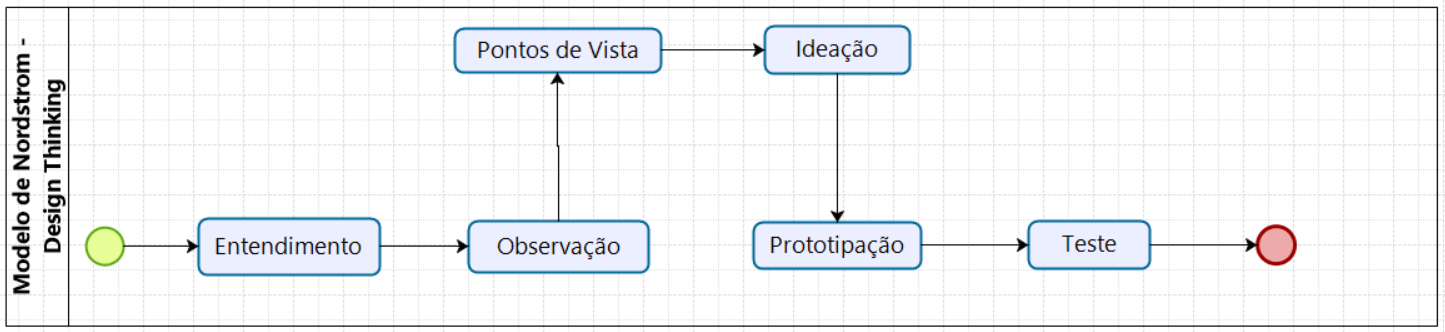
\includegraphics[width=1.00\textwidth]{img/modelo_6fases_DT.png}
% \caption{Modelo de Nordstrom - Design Thinking \cite{kabiawu2016designing}}
% \label{fig:modelo6fasesdt}
% \end{figure}
% \todo[inline]{se vc for falar de indicadores de requisitos é bom referenciar o trabalho da carla silva de DT e requisitos, ela vai participar da sua banca provavelmente porque é a area dela, dá uma olhada:Cynara Souza, Carla Silva:
% Uso do design thinking na elicitação de requisitos de ambientes virtuais de aprendizagem móvel. CIbSE 2014: 561-574
% }

% \subsection{Design Sprint}

% Segundo Ghanim e Phaal \cite{DBLP:conf/ice-itmc/Al-AliP19}, O \textit{Design Sprint} foi adaptado de várias práticas de design utilizados pela industria, incluindo o \textit{Design Thinking}. O \textit{Design Sprint} é uma metodologia para resolver problemas e testar ideias em um processo rápido. Segundo os autores, o processo de \textit{Design Sprint} é um workshop de um a cinco dias, que vai rapidamente da compreensão do desafio ao teste de soluções com os usuários. O Design Sprint possui seis etapas:

% \begin{itemize}
%     \item \textbf{Compreender} o desafio e desenvolver uma base de conhecimento compartilhada entre os participantes;
%     \item \textbf{Definir} o contexto e os resultados desejados para estabelecer o foco;
%     \item \textbf{Esboçar} uma ampla gama de ideias a serem consideradas ainda mais e refinadas;
%     \item \textbf{Decidir} e finalizar a direção ou conceito a ser prototipado;
%     \item \textbf{Prototipar} um conceito de baixa fidelidade suficiente para validar as hipóteses;
%     \item \textbf{Validar} as descobertas com usuários reais ou partes interessadas.
% \end{itemize}

% \todo[inline]{o trabalho do Vinicius tem um desenho muito bom do DS e pode te ajudar a melhorar, posso compartilhar a dissertacao dele contigo}

% \subsection{Comparação entre Design Thinking e Design Sprint}

% A primeira vista, percebe-se várias semelhanças entre o \textit{Design Thinking} e o \textit{Design Sprint}. Contudo, alguns aspectos conceituais e o contexto de utilização tornam as duas abordagens diferentes. As diferenças e comparações são abordadas por Mendonça et al \cite{DBLP:conf/hci/AraujoSCA19}. Este objeto de estudo descreve um estudo comparativo, conforme apresentado na Figura \ref{fig:comp_ds_dt}, das duas metodologias usadas para minimizar os problemas enfrentados pelas empresas na obtenção dos requisitos de seu software, apresentando suas fases e como elas podem ser usadas. Percebe-se que a primeira diferença está no conceito de cada abordagem:

% \begin{itemize}
%     \item \textbf{Design Thinking:} É uma metodologia que contrasta com a metodologia científica tradicional, na qual se baseia na colaboração de uma equipe multidisciplinar para resolver problemas complexos através da aplicação do conhecimento de design \cite{DBLP:conf/hci/AraujoSCA19};
%     \item \textbf{Design Sprint:} É um processo exclusivo do Google Venture de cinco dias usado para resolver problemas críticos por meio de prototipagem e \textit{brainstorming} com os clientes. Todas as melhores ideias são condensadas e organizadas em um curto espaço de tempo para a criação de uma excelente ideia. Nesse processo, uma descrição passo a passo do que deve ser feito em cada um desses cinco dias é fornecida em detalhes. No final desses cinco dias, cria-se um produto validado em que acredita-se que o projeto, da maneira como foi projetado, não é ideal \cite{DBLP:conf/hci/AraujoSCA19}.
% \end{itemize}

% Segundo os autores, é necessário entender o contexto no qual o nível de maturidade da ideia se encontra, antes de escolher qual a melhor abordagem a ser adotada para o problema a ser analisado.
% \begin{itemize}
%     \item Se é necessário desenvolver soluções ou criar algo totalmente novo, é melhor optar pelo \textit{Design Thinking}, uma abordagem focada em imergir e entender um contexto holístico em que um problema complexo está incorporado. Agora, se seu objetivo é co-criar a equipe para encontrar a solução viável, o \textit{Design Sprint} é mais recomendado, pois é mais objetivo no processo \cite{DBLP:conf/hci/AraujoSCA19};
%     \item Um dos grandes vilões da inovação é talvez o momento, tanto pela dedicação que sua equipe precisa ter quanto pelo nível de inovação que deve apresentar. Se a equipe precisar desenvolver a solução ou pelo menos um produto mínimo viável (MVP) rapidamente, o \textit{Design Sprint} é recomendado. Agora, se a ideia é entender o contexto em profundidade e criar uma solução, o \textit{Design Thinking} cumpre bem esse papel \cite{DBLP:conf/hci/AraujoSCA19};
%     \item Embora as duas abordagens sejam baseadas em colaboração e experimentação, o \textit{Design Thinking} tem um caráter mais "aprender compartilhando", uma vez que o Design Sprint é mais "aprender fazendo" devido ao tempo dos sprints e à velocidade necessária para criar um MVP. Tanto o \textit{Design Thinking} quanto o \textit{Design Sprint} são abordagens que alavancam significativamente a capacidade das pessoas envolvidas em serem criativas. De fato, ambas as abordagens são caracterizadas por ferramentas e metodologias que dão suporte à geração de ideias. A metodologia \textit{Design Sprint} promove uma abordagem mais crítica, proporcionando um número maior de sessões dedicadas ao pensamento individual em comparação ao sugerido pelo \textit{Design Thinking} \cite{DBLP:conf/hci/AraujoSCA19}.
% \end{itemize}

% \begin{figure}[htb!]
% \centering
% 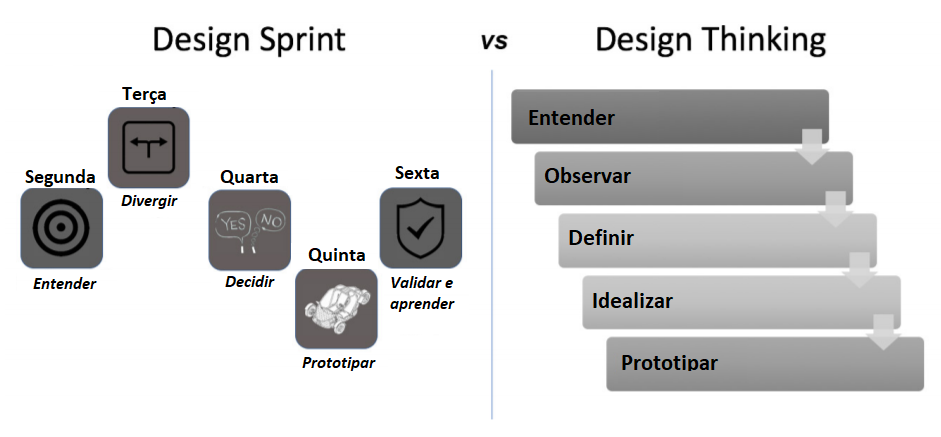
\includegraphics[width=0.90\textwidth]{img/ds_dt.png}
% \caption{Comparativo entre Design Thinking e Design Sprint \cite{DBLP:conf/hci/AraujoSCA19}}
% \label{fig:comp_ds_dt}
% \end{figure}

% Com relação ao trabalho proposto, optou-se por utilizar tanto o \textit{Design Thinking} quanto o \textit{Design Sprint}, tendo em vista que a proposta do modelo envolve a criação de algo novo, juntamente com a aplicação de um processo de co-criação entre os membros da equipe para encontrar uma solução viável. Existe também a necessidade de se entender o escopo do problema de forma profunda e gerar um MVP o mais rápido possível, com o intuito de se conseguir o patrocínio da alta direção, para a aplicação do modelo.

% \subsection{Cynefin}

% Além do \textit{Design Thinking} e \textit{Design Sprint}, com foco exclusivo nas necessidades do usuário, outras abordagens surgiram para apoiar a tomada de decisão estratégica da organização. Um \textit{framework} muito utilizado neste contexto nos dias atuais é o Cynefin \cite{shalbafan2018decision}. De acordo com Snowden e Boone \cite{snowden2007leader}, a ideia do Cynefin é oferecer aos tomadores de decisão um modelo a partir do qual eles podem ver suas percepções. Os autores utilizam o termo para se referir à ideia de que todos temos conexões e estamos inseridos em um ou mais sistemas. Cada sistema está inserido em um ou mais contextos ou domínios e, dependendo do contexto, diferentes ações serão executadas para resolver determinados problemas. O Cynefin define quatro domínios, conforme apresentado na Figura: \ref{fig:cynefin-framework}:

% \begin{itemize}
%     \item \textbf{Óbvio:} O domínio óbvio representa os sistemas conhecidos. Isso significa que existem regras em vigor (ou melhores práticas), a situação é estável e a relação entre causa e efeito é clara: se você faz X, espera Y. O conselho nessa situação é definir um sentido, categorizar e responder, seguindo a regra ou aplicando as melhores práticas;
%     \item \textbf{Complicado:} O domínio complicado consiste em "conhecer o desconhecido". A relação entre causa e efeito requer análise ou perícia. Há várias respostas corretas. A estrutura recomenda definir um sentido, analisar e responder. Avaliar os fatos, analisar e aplicar as boas práticas operacionais apropriadas;
%     \item \textbf{Complexo:} O domínio complexo representa as "incógnitas desconhecidas". Causa e efeito só podem ser deduzidos em retrospecto, não há respostas corretas e padrões instrutivos podem surgir. Neste domínio, há muita pesquisa e experimentação com foco no problema a ser analisado. Neste domínio, a estrutura recomenda examinar, definir um sentido e responder;
%     \item \textbf{Caótico:} No domínio caótico, causa e efeito não são claros. Segundo Snowden e Boone \cite{snowden2007leader}, os eventos neste domínio são muito confusos para esperar por uma resposta baseada no conhecimento. Ação (qualquer ação) é a primeira e única maneira de responder adequadamente. Neste contexto, os gerentes agem e respondem. Agem para estabelecer a ordem; sentir onde está a estabilidade; e respondem para transformar o caótico no complexo.
% \end{itemize}

% \begin{figure}[htb!]
% \centering
% 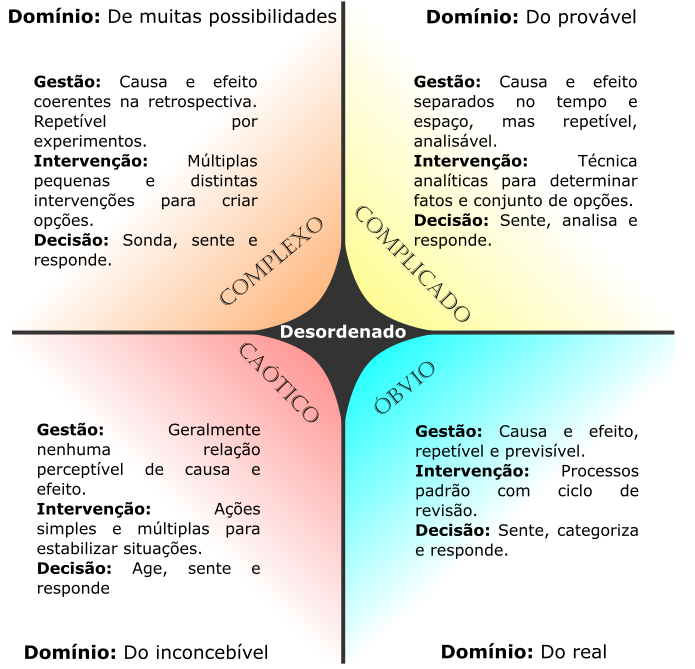
\includegraphics[width=0.80\textwidth]{img/Cynefin_Fred.png}
% \caption{Cynefin Framework \cite{shalbafan2018decision}}
% \label{fig:cynefin-framework}
% \end{figure}

% \section{Estágios de Evolução na Eficiência da Priorização e Definição de Indicadores}

% O conceito de métricas e indicadores sempre acompanhou as etapas evolutivas da nossa sociedade. Segundo Memória \cite{memoria2004breve}, os primeiros indicadores surgiram na época do império romano, com a necessidade de se mensurar as dimensões sociais como a idade da população e morte. Indicadores do panorama da população eram elementos importantes de definição das riquezas e poder do Estado. Em seguida, as estatísticas econômicas começaram a ser coletadas, principalmente no início da revolução industrial \cite{schwab2019quarta}.  No início da história e da evolução dos indicadores, predominava a exclusiva quantificação, seja de pessoas, recursos ou equipamentos \cite{memoria2004breve}. 
    
% Após a consolidação dos indicadores sociais, surgiu-se a necessidade de se definir indicadores econômicos, como o Produto Interno Bruto (PIB), utilizado para mensurar o nível de riqueza de uma nação. Seguindo o panorama evolutivo na gestão de indicadores, segundo Gonçalves \cite{gonccalves2000empresas}, no século XX surgiu a ideia de organizações orientadas por processo. Estrutura organizacionais passaram a definir como produtos e serviços seriam oferecidos aos seus usuários por meio de um sequenciamento de atividades que recebe uma ou mais entradas e retornam uma ou mais saídas. Novamente era necessário nos adaptarmos para definir como poderíamos medir o grau de  eficiência e eficácia de organizações orientadas por processo. Neste contexto, surgiu a definição dos KPI's -- \textit{Key Performance Indicators}. Segundo Shahin e Mahbod \cite{shahin2007prioritization} definir KPI's adequados para as necessidades da organização é essencial para que ela consiga otimizar os resultados dos seus processos. Ainda segundo os autores, além de definir, é necessário priorizar quais indicadores precisam ser melhorados para agregar mais valor a organização. Para isso, eles definiram uma abordagem integrada que prioriza os KPI's em termos dos critérios de definição de metas SMART \textit{(Specific, Measurable, Attainable, Realistic, Time‐sensitive)}.
    
% As mudanças acontecem de forma exponencial, por isso é necessário adaptar e descobrir novas formas de mensurar os processos organizacionais. Definir e priorizar métricas e indicadores através da visão da alta direção não garante que a expectativa dos usuários finais serão plenamente atendidas. É necessário entender as reais necessidades do usuário final, se colocar em seu lugar e tentar perceber quais indicadores agregarão mais valor às suas necessidades. Portanto, uma nova abordagem para mensurar e definir indicadores deve ser desenvolvida, com o foco exclusivo nas necessidades do usuário final \cite{bertoni2017systematic}, \cite{canedodesign}.
  
%   \todo[inline]{todos estes indicadores estão detalhados no texto? o seu texto está muito bom FRed essas sugestões são para ficar melhor ainda e nao deixar a banca na duvida, acho que se é imperio romano ou transformação digitacao vc pode colocar em outro lugar sem ser no nome da coluna por exemplo que tal vc colocar as seguintes colunas: ID Tipo Descrição Lista de Indicadores  -- ai por exemplo vc vai listar os sociais e na descricao vc diz que é do IR}  
% \begin{table}[!htpb]
% 	\centering
% 	\caption{Tipos de Indicadores Encontrados na Literatura}
% 	\begin{center}
% 		\begin{tabular}{|p{3.0cm}|p{2.5cm}|p{2.5cm}|p{2.5cm}|p{3.0cm}|}
% 			\hline
% 			\textbf{Tipo}  & \textbf{Império Romano (Século I)}  &\textbf{Revolução Industrial (Século XVIII)} &\textbf{Organizações corporativas (Século XX)} &\textbf{Transformação Digital (Século XXI)}\\
% 			\hline\hline
% 			Indicadores Sociais \cite{nations2014united} &X &X &X &X\\
% 			\hline
% 			Indicadores econômicos \cite{nations2014united} & &X &X &X\\
% 			\hline
% 			Indicadores de performance (KPI) \cite{costoiu2016environmental} & & &X &X\\
% 			\hline
% 			Indicadores de Inovação \cite{mesquita2018inteligencia} & & & &X\\
% 			\hline
% 		\end{tabular}
% 		\label{tab:cronograma2}
% 	\end{center}
% \end{table} 
    
%     \todo[inline]{FRED se for indicadores apenas para requisitos acho falta definir requisitos e os tipos. no inicio da seção 2.1 vc coloca os tipos diferentes de categorias de indicadores para requisitos, então antes defina req e etc. Pegue uma referencia classica da conferencia de RE e talvez dos artigos da carla silva}
    
% \subsection{Aplicação da Gestão de Indicadores nas Organizações}

% A gestão de indicadores é uma tendência crescente na atualidade. Particularmente, a gestão de indicadores nas organizações vem transformando o relacionamento entre o usuário final e empresa. Esse processo tem sido visto como uma grande oportunidade para as empresas garantirem a satisfação plena dos usuários, ofertando produtos e serviços com mais qualidade e agilidade, promovendo assim a perenidade do relacionamento entre o cliente e a organização \cite{kozak2006relationship}.

% Apesar dos benefícios serem inquestionáveis \cite{alemanni2008key} \cite{DBLP:journals/chb/JetterER18} \cite{niemann2017benefits}, as formas de se definir e priorizar indicadores são variadas, sendo que cada organização, de acordo com suas metas e possibilidades, adota práticas distintas e variadas. Portanto, é uma tarefa complexa estabelecer comparações entre as organizações quanto ao nível de maturidade da gestão de indicadores. Avaliando o contexto das organizações no Brasil, observam-se algumas iniciativas das organizações brasileiras com a \textbf{definição e priorização mais eficiente de indicadores de performance}, com a construção de programas, diretrizes e apoio institucional. 

% A Estratégia de gestão de indicadores da Petrobrás \cite{de2010processo} define os objetivos estratégicos, metas e indicadores por meio do Balanced Scorecard (BSC) \todo[inline]{coloque a referencia de BSB tambem} e afirma que seu principal desafio é cultural. O BSC resume e indica em um único documento o desempenho de quatro perspectivas: financeiro, clientes, processos internos e aprendizado e crescimento. Segundo os autores, este estudo é importante porque o BSC é a primeira tentativa sistemática de desenvolver um projeto para um processo de avaliação de desempenho focado nos objetivos da empresa, na coordenação de decisões individuais e na base do aprendizado organizacional com a intenção de explorar, potencializar e orquestrar sinergias que promovam maior eficácia, eficiência, efetividade e economicidade para a organização. A gestão de indicadores pretende auxiliar os tomadores de decisão da organização a entenderem quais indicadores trará um benefício mais significativo para o seu cliente, com melhorias no ambiente de negócios e com eficiência da gestão organizacional \cite{de2010processo}.

% Neste cenário de constantes mudanças, as organizações preveem que a gestão adequada e eficiente de indicadores se torne essencial para a sua sobrevivência nos próximos anos. Para isso, uma das iniciativas compreende a entender sobre qual indicador a organização deverá focar para conseguir agregar mais valor para o usuário final.

% \todo[inline]{aqui qual indicador organização deverá focar -- ficou generico, se vc for focar em tipo especifico, coloque. Neste trabalho o nosso foco são nos indiciadores de requisitos ou de gestao de projetos, ou de melhoria de processos, processos de negócios,etc......}

% \subsection{Trabalhos Correlatos}

% Gerenciar indicadores é uma tarefa essencial para alcançar os objetivos estratégicos de uma organização. A medição do grau de eficiência dos processos e projetos para o alcance destes objetivos fornece para a organização informações essenciais para a tomada de decisão na direção correta. Sanchez \cite{sanchez2015integrating} propõe uma integração entre as questões de sustentabilidade ao gerenciamento de projetos. Segundo Sanchez \cite{sanchez2015integrating}, é necessário desenvolver uma estrutura para ajudar a garantir que uma organização esteja trabalhando nos projetos certos para atingir sua estratégia de negócios e as demandas das partes interessadas. Para isso, a proposta do autor aborda o problema relacionado a seleção de portfólio e ao rastreamento do projeto. O autor utiliza o Balanced Scorecard (BSC) \cite{kaplan1992balanced} e seus respectivos indicadores para mensurar o impacto da sustentabilidade na definição e monitoramento do portfólio de projetos.

% Alguns autores sugerem diferentes abordagens para aprimorar os processos de negócio de uma organização, com base em indicadores. Segundo González et al. \cite{sanchez2017case}, as organizações estão cada vez mais preocupadas com a melhoria do modelo de processos de negócios em seus esforços para garantir maior eficiência operacional, entretanto, realizar a avaliação dos resultados da medição não é uma tarefa simples e requer a identificação de indicadores e \textit{threshold} relevantes, capazes de distinguir diferentes níveis de qualidade do modelo de processo. Para isso, os autores apresentaram um estudo de caso para avaliar o \textit{framework} BPMIMA (melhoria do modelo com base nas atividades de medição) para melhoria do modelo de processos de negócio, conforme apresentado na Figura \ref{fig:bpmime}. Essa estrutura é composta por medições que são empiricamente validadas e estão relacionadas às características de qualidade dos modelos, um conjunto de indicadores com limites validados associados às diretrizes de modelagem e uma ferramenta de suporte a prototipação. Para validar a eficácia potencial do BPMIMA na prática, os autores aplicaram o modelo em um estudo de caso representativo do setor da saúde, no Hospital General Universitário de Ciudad Real, na Espanha. Segundo os autores, os resultados obtidos neste estudo de caso sugerem fortemente que a aplicação de indicadores poderia detectar modelos não adequados sob uma perspectiva de compreensibilidade e modificabilidade. Portanto, a aplicação de indicadores e diretrizes nos modelos de processos hospitalares indica percepções fortes e favoráveis de melhorias na qualidade \cite{sanchez2017case}.

% \begin{figure}[htb!]
% \centering
% 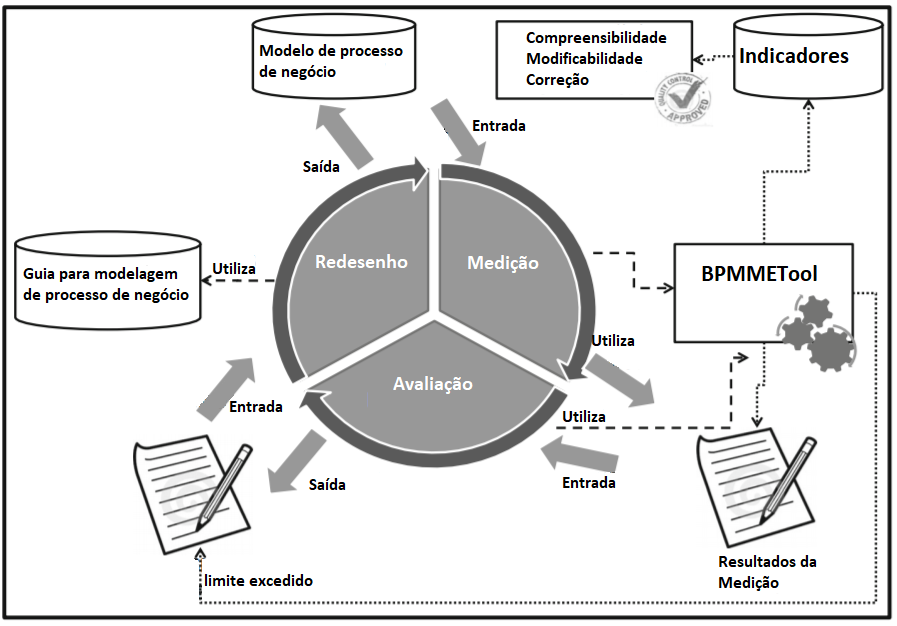
\includegraphics[width=0.9\textwidth]{img/BPMIMA.png}
% \caption{Framework BPMIME (tradução nossa) \cite{sanchez2017case}}
% \label{fig:bpmime}
% \end{figure}

% Outros autores optaram por restringir o escopo de pesquisa e focar apenas em um grupo específico de indicadores, como é o caso de Wang et al. \cite{wang2016practical} que define um guia prático para selecionar indicadores de qualidade para algoritmos de pesquisa baseado em Pareto \todo[inline]{referenciar pareto}. Segundo os autores, um dos principais desafios da aplicação de algoritmos de pesquisa baseados em Pareto é selecionar indicadores de qualidade apropriados, por exemplo, \textit{hipervolume}, para avaliar a qualidade das frentes de Pareto. Para isso, os autores avaliaram oito indicadores de qualidade de quatro categorias diferentes com seis algoritmos de busca baseados em Pareto e, com base nos resultados dos experimentos, definiram um guia prático.

% Em um estudo empírico realizado por Qiao et al. \cite{qiao2018empirical}, os autores investigaram a definição de indicadores de envelhecimento de software no Android, concentrando-se em indicadores de envelhecimento, como memória física livre do sistema e memória de pilha do aplicativo. Os autores analisaram os resultados com métricas de avaliação tradicionais como MAPE (\textit{Mean Absolute Percentage Error}) / MSE (\textit{Mean Squared Error}) para avaliar todo o desempenho da previsão e com nossas métricas de avaliação propostas TA (\textit{trend accuracy}), FA (\textit{fluctuation accuracy}), SVA (\textit{small variation accuracy} \todo[inline]{Fred sempre coloca por extenso primeiro e depois a sigla, corrigir em todo o texto -- texto (TE)}) para avaliar a tendência, flutuação e pequena variação dos indicadores de envelhecimento, respectivamente.

% Percebe-se que os autores supracitados \todo[inline]{(REVISADO) vc citou 3 acima, se são varios coloque as referencias} desenvolveram suas pesquisas com o objetivo de definir indicadores em contextos bem específicos dentro das organizações. No entanto, não há um objeto de estudo que tente propor uma solução para a definição e priorização de indicadores \todo[inline]{(REVISADO) que tipo de indicadores? Fred: Não há um tipo específico de indicadores. O modelo propõe a definição e priorização de indicadores em qualquer escopo -- Edna Acho que essa explicação deve ficar então no final desse texto explicando isso e dizendo o que fará em um escopo x senao seu trabalho ficará muito aberto, pelo que entendo vc fara em desenvolvimento de sw certo?} utilizando uma abordagem com ênfase na criatividade e inovação. Definir uma abordagem com o foco em inovação se tornou vital para que as organizações consigam se adaptar ao rápido ciclo de mudanças no mundo. Segundo Bessant e Tidd \cite{tidd2015gestao}, a inovação é o serviço que entregue valor, dentro de uma nova experiência, e este valor faz alterar o comportamento dos usuários. Segundo os autores, para o sucesso da execução da inovação, é necessário definir uma estratégia para aplicação da inovação na organização e, dentro desta estratégia, é necessário definir as fontes de inovação, as redes (conexões) de inovação e uma estratégia da implantação do plano de inovação da organização.

    
% Um estudo realizado apenas com empresas brasileiras, demonstrou a importância de uma gestão adequada de indicadores para o sucesso dos projetos de TIC. Berssaneti e Carvalho \cite{berssaneti2015identification} buscaram identificar as variáveis que impactam o sucesso do projeto em empresas brasileiras. Dentre algumas variáveis identificadas, destaca-se a importância de mensurar de forma adequada e transparente o progresso do projeto. Portanto, a gestão adequada de indicadores é um fator preponderante para o sucesso dos projetos.
    
% Todorovic et al. \cite{todorovic2015project} propuseram um \textit{framework} para análise de sucesso de projetos. O \textit{framework} foi definido com base em dados coletados da percepção de 103 gerentes de projetos em diferentes setores da indústria. Os resultados encontrados confirmaram que a análise de sucesso de projetos, apresentada através da definição de fatores críticos de sucesso, indicadores-chave de desempenho (KPIs) e processo de medição de desempenho, tem uma influência muito positiva na aquisição de conhecimento no ambiente do projeto.

% Alguns trabalhos abordaram a questão da definição de indicadores em um contexto mais específico, como por exemplo, a infraestrutura de TIC. De acordo com Benitez et al. \cite{benitez2018impact} é muito importante que a infraestrutura tecnológica das empresas seja flexível para se adaptar ao processo de fusão e/ou aquisição (M\&A). Segundo os autores, as fusões e aquisições permitem que as empresas alcancem sinergias baseadas em custos por meio de economia de escala e escopo. As fusões e aquisições também permitem que as empresas obtenham sinergias baseadas em receita, alavancando os principais recursos. Dessa forma, é de extrema importância que se defina indicadores adequados para mensurar o grau de eficiência na execução do processo de M\&A. Para isso, os autores propuseram alguns indicadores, como, por exemplo, o indicador que mediu as atividades de M\&A através do logaritmo natural do número de M\&A por empresa, o indicador perceptivo de vendas, indicador de capacidade de integração de TIC pós-M\&A e o indicador de performance de M\&A.
    
% Algumas pesquisas relacionadas a gestão de indicadores decidiram focar em aspectos conceituais do tema; como, por exemplo, o objeto de estudo desenvolvido por Dominguez et al \cite{DBLP:journals/csi/DominguezPRZ19} que busca aprimorar o entendimento do gerenciamento de KPIs e ajudar os usuários a decidir sobre a solução mais adequada para as suas necessidades. A pesquisa desenvolvida pelos autores possui duas abordagens distintas. Com relação ao processo iterativo, o método distingue duas abordagens: \textit{indutiva ou empírica-conceitual}, que é apropriada quando os pesquisadores têm pouco entendimento do domínio, mas há dados significativos sobre os objetos disponíveis e \textit{dedutiva ou conceitual-empírica}, que é aconselhável se houver poucos dados disponíveis, mas os pesquisadores tiverem uma compreensão significativa do domínio. A taxonomia proposta pelos autores abrange os aspectos gerais considerados por outras propostas e que captura mais completamente as características únicas do gerenciamento de KPIs (focando principalmente na definição de KPIs). A taxonomia resultante estabelece cinco dimensões relacionadas ao gerenciamento de KPIs, tentando responder as seguintes perguntas:

% \begin{enumerate}
%     \item \textit{O que é medido por um KPI?} Visa esclarecer os diferentes aspectos a serem medidos pelos KPIs;
%     \item \textit{Quais recursos são considerados na especificação de KPIs?} Aborda os diversos e variados recursos que podem ser considerados na especificação de KPIs;
%     \item \textit{Para que um KPI é medido?} A intenção é identificar os diferentes propósitos para os quais um KPI pode ser usado;
%     \item \textit{Quais artefatos são usados para design e especificação de KPI?} Visa esclarecer os tipos de elementos comumente usados para criar KPIs;
%     \item \textit{Quais são as características de uma abordagem de gerenciamento de KPIs?} Aborda as diferentes particularidades para gerenciar KPIs usados pelas propostas existentes.
% \end{enumerate}

% \begin{figure}[htb!]
% \centering
% 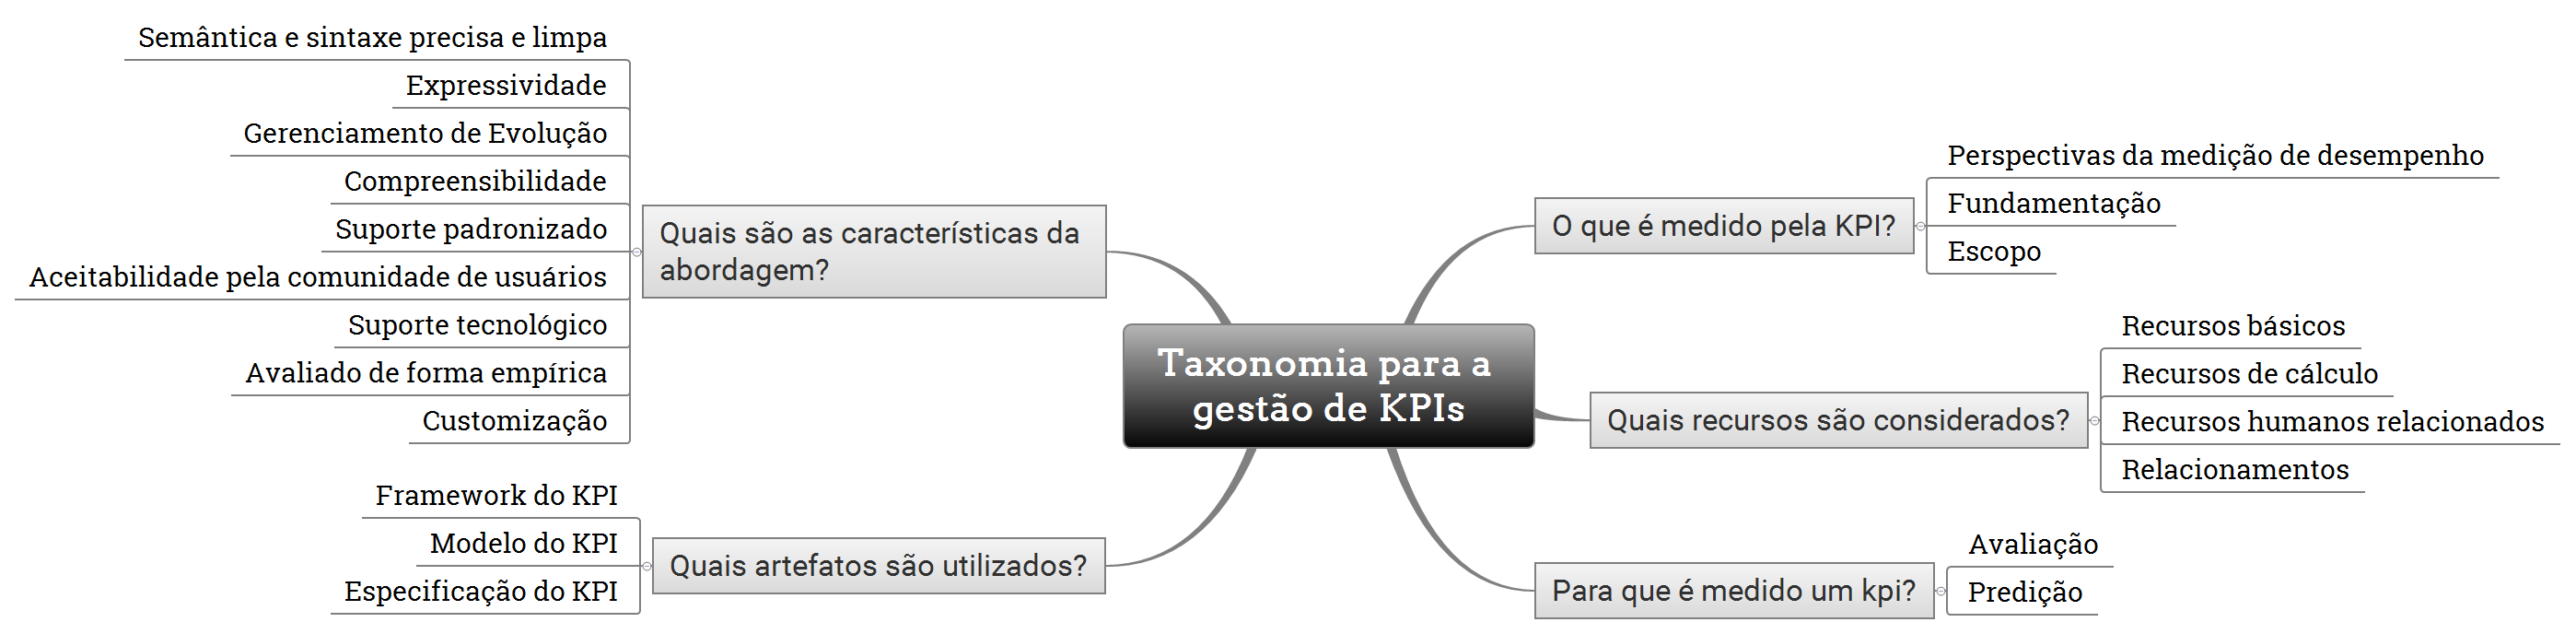
\includegraphics[width=1.0\textwidth]{img/taxonomia_ptBR.png}
% \caption{Taxonomia para o gerenciamento de KPIs (tradução nossa) \cite{DBLP:journals/csi/DominguezPRZ19}}
% \label{fig:taxonomiagestaokpis}
% \end{figure}

% Outros autores optaram por pesquisar especificamente um modelo de avaliação de indicadores. O trabalho apresentado por Kucukaltan e Topcu \cite{DBLP:journals/jeim/KucukaltanT19} propôs definir um modelo de avaliação dos principais indicadores de seleção de companhias aéreas em um modelo de decisão estratégica. Segundo os autores, estruturar o modelo de decisão estratégica a partir do conjunto de indicadores é vital para se obter um modelo de decisão estratégia adequado e aderente às necessidades da organização. 

% De acordo com Mesquita e Janissek \cite{mesquita2018inteligencia}, o uso do conceito de Inteligência Estratégica já é uma realidade entre as empresas, gerando informações importantes para a criação de vantagem competitiva, ao passo que o conceito de Design Thinking é utilizado como um método para satisfazer objetivos econômicos e criativos. Ambos os conceitos possuem etapas de processo que os caracterizam como cíclicos e que estão diretamente ligados à estratégia da organização. Da Silva \cite{da2018design} utilizou o Design Sprint em um estudo de caso no qual se avaliou o nível de engajamento de equipes de design. O estudo de caso de aplicação dessa metodologia envolveu a participação de um professor e um grupo de 75  estudantes.

% Segundo Juhnke et al. \cite{DBLP:conf/se/JuhnkeTH18}, o teste é uma atividade importante de garantia de qualidade durante o desenvolvimento de software automotivo. Dessa forma, os autores propuseram 7 indicadores potenciais de qualidade:
% \begin{itemize}
%     \item Tamanho da especificação do caso de teste com relação à especificação de requisitos;
%     \item Distribuição de tipos de objetos contidos;
%     \item Tamanho dos casos de teste;
%     \item Tipo de especificação de caso de teste;
%     \item Tipo de tipos de objetos vinculados;
%     \item Número de tipos de objetos vinculados;
%     \item Percentual de conformidade do \textit{template}.
% \end{itemize}

% Além dos indicadores supracitados, há a necessidade de se definir indicadores para mensurar o risco de um determinado projeto ou processo. A partir desta premissa, Kumar et al. \cite{rai2017identification} propôs a identificação de indicadores de risco de software ágil em projetos de desenvolvimento de software ágil. Segundo os autores, a utilização de indicadores de risco é útil para planejar a avaliação de riscos em qualquer projeto de software ágil que esteja planejando desenvolver. É útil para otimização de processos e ajuda nas decisões gerenciais. Apesar da importância do gerenciamento de riscos em projetos de software, esta prática ainda é geralmente ignorada pelas organizações que desenvolvem software ágil. Uma razão para esse fato é que o conceito de risco não é configurável e distorcido, e sua gestão não traz resultados práticos imediatos visíveis. Para obter um resultado satisfatório na execução do processo de gestão de riscos, é necessário indicadores de risco para um ou mais elementos de risco que foram identificados no projeto \cite{rai2017identification}. A Tabela \ref{tab:indicadoresdesenvolvimentoagil} apresenta uma lista de elementos de riscos, assim como o indicador que mensura cada elemento identificado.

% \begin{center}
% \begin{longtable}{|p{7.0cm}|p{8.0cm}|}
%     \caption{Riscos no Desenvolvimento Ágil \cite{rai2017identification}}\\
%     \hline 
%     \multicolumn{1}{|c|}{\textbf{Indicadores de Risco}} & \multicolumn{1}{c|}{\textbf{Elementos de Risco}} \\ \hline 
%     \endfirsthead
%     \multicolumn{2}{c}%
%     {{\bfseries \tablename\ \thetable{} -- Riscos no Desenvolvimento Ágil}} \\
%     \hline 
%     \multicolumn{1}{|c|}{\textbf{Indicadores de Risco}} & \multicolumn{1}{c|}{\textbf{Elementos de Risco}} \\ \hline 
%     \endhead
%     \hline 
%     \endfoot
%     \hline 
%     \endlastfoot
% 	\hline
% 			\multirow{2}{*}{Riscos do ambiente de desenvolvimento} 
% 			    & Larga escala, \textit{offshore} e distribuído.\\
% 			    \cline{2-2}
% 			    & A função do \textit{Product Owner} (PO) não está preenchida corretamente.\\
% 			    \cline{2-2}
% 			    & As equipes não estão focadas.\\ 
% 			    \cline{2-2}
% 			    & Falta de apoio do patrocinador.\\ 
% 			    \cline{2-2}
% 			\hline
% 			\multirow{2}{*}{Riscos de Problemas de Processo} 
% 			    & Os membros da equipe se inscreveram no processo do software, pois ele é documentado por meio da metodologia ágil e estão dispostos a usá-lo.\\ 
% 			    \cline{2-2}
% 			    & Padrões de engenharia de software ágil não fornecidos para todo desenvolvedor e gerente de software.\\
% 			    \cline{2-2}
% 		    \hline
% 		    \multirow{2}{*}{Tamanho e experiência da equipe} 
% 			    & As melhores pessoas não disponíveis para equipes auto-organizadas.\\
% 			    \cline{2-2}
% 			    & As pessoas não têm a combinação certa de habilidades.\\
% 			    \cline{2-2}
%                 & A equipe não está comprometida por toda a duração do projeto.\\
%             \hline
%             \multirow{2}{*}{Riscos de Problemas Técnicos} 
% 			    & Técnicas de especificação de aplicativos facilitadas não são usadas para auxiliar na comunicação entre o cliente e o desenvolvedor do software ágil.\\
% 			    \cline{2-2}
% 			    & Métodos específicos não estão disponíveis para análise de software ágil.\\
% 			    \cline{2-2}
%                 & Métodos específicos não estão disponíveis para o design do caso de teste.\\
%             \hline
%             \multirow{2}{*}{Riscos tecnológicos} 
% 			    & Tecnologia a ser construída nova para sua empresa.\\ 
% 			    \cline{2-2}
%                 & A interface do software com hardware novo ou não comprovado. O software a ser construído faz interface com um sistema de banco de dados cuja função e desempenho não foram comprovados nesta área de aplicação.\\
%              \hline
% 			 \multirow{2}{*}{Risco de cronograma} 
% 			    & A programação, os recursos e a definição do produto foram todos ditados pelo cliente ou pela gerência superior.\\
% 			    \cline{2-2}
% 			    & O cronograma é otimista, "melhor caso", em vez de realista, "caso esperado".\\ 
% 			    \cline{2-2}
%                 & O cronograma não aprovado pelos membros da equipe específicos que desempenharão o papel principal.
%     \label{tab:indicadoresdesenvolvimentoagil}
% 	\end{longtable}
% \end{center}

% Diferentemente dos trabalhos correlatos, neste trabalho iremos propor um modelo; composto por abordagens focadas na criatividade e solução de problemas complexos, como o \textit{Design Thinking}, \textit{Design Sprint} e \textit{Cynefin}; para a definição e priorização de indicadores. A priorização ocorrerá no contexto em que a organização já possui uma lista de indicadores, porém, não sabe qual desses indicadores, ao serem otimizados, gerará um impacto mais positivo na organização. A definição ocorrerá no contexto em que a organização concluiu que nenhum dos indicadores definidos e monitorados por ela, caso sejam otimizados, gerarão um impacto suficientemente positivo. Neste caso, será necessário definir e otimizar um novo indicador, a ser verificado após a execução do modelo. 

% \section{Síntese do Capítulo}

% Este capítulo apresentou os conceitos necessários para o entendimento do contexto desta dissertação, os quais foram: \textbf{Design Thinking} -- abordagem utilizada para solucionar problemas complexos, sendo apresentado também o conceito de \textit{Design Sprint} (processo desenvolvido pelo Google Ventures, com atividades mais restritas e menos adaptativas); \textbf{Cynefin} -- \textit{framework} para categorizar o problema em domínios e propor uma diretriz para solucioná-lo e \textbf{Indicador} -- mecanismo utilizado para mensurar o desempenho de processos e projetos. Além disso, foram apresentados alguns trabalhos correlatos à este, mostrando os seus principais diferenciais.

% \todo[inline]{(Esse parágrafo aqui é no início do 3.}

% Este capítulo apresenta o modelo proposto, que tem como objetivo identificar quais indicadores devem ser priorizados pela organização, para otimização, por meio de um projeto ou plano de ação, com o intuito de prover produtos e serviços com qualidade e tornar os processos de negócio mais eficientes. O modelo terá como entrada uma lista de indicadores previamente filtrados e analisados (Tabela \ref{tab:indicadoresanalisados}), e terá como saída uma nova lista de indicadores a serem otimizados, priorizados por ordem de importância, de acordo com o processo definido na Figura: \ref{fig:processo_modelo}.






